\chapter{Analisi dei risultati sperimentali}
\label{capitolo4}
\thispagestyle{empty}

In questo capitolo discutiamo i risultati degli algoritmi da noi selezionati sui dati raccolti.

\section{LAC}
Le prestazioni dell'algoritmo sono visibilmente influenzate dal numero di cluster e dal valore assegnato al parametro \textit{h} (\autoref{fig:lac_correlation_1500}.
\begin{figure}[h]
        \centering
        \begin{subfigure}[b]{0.85\textwidth}
                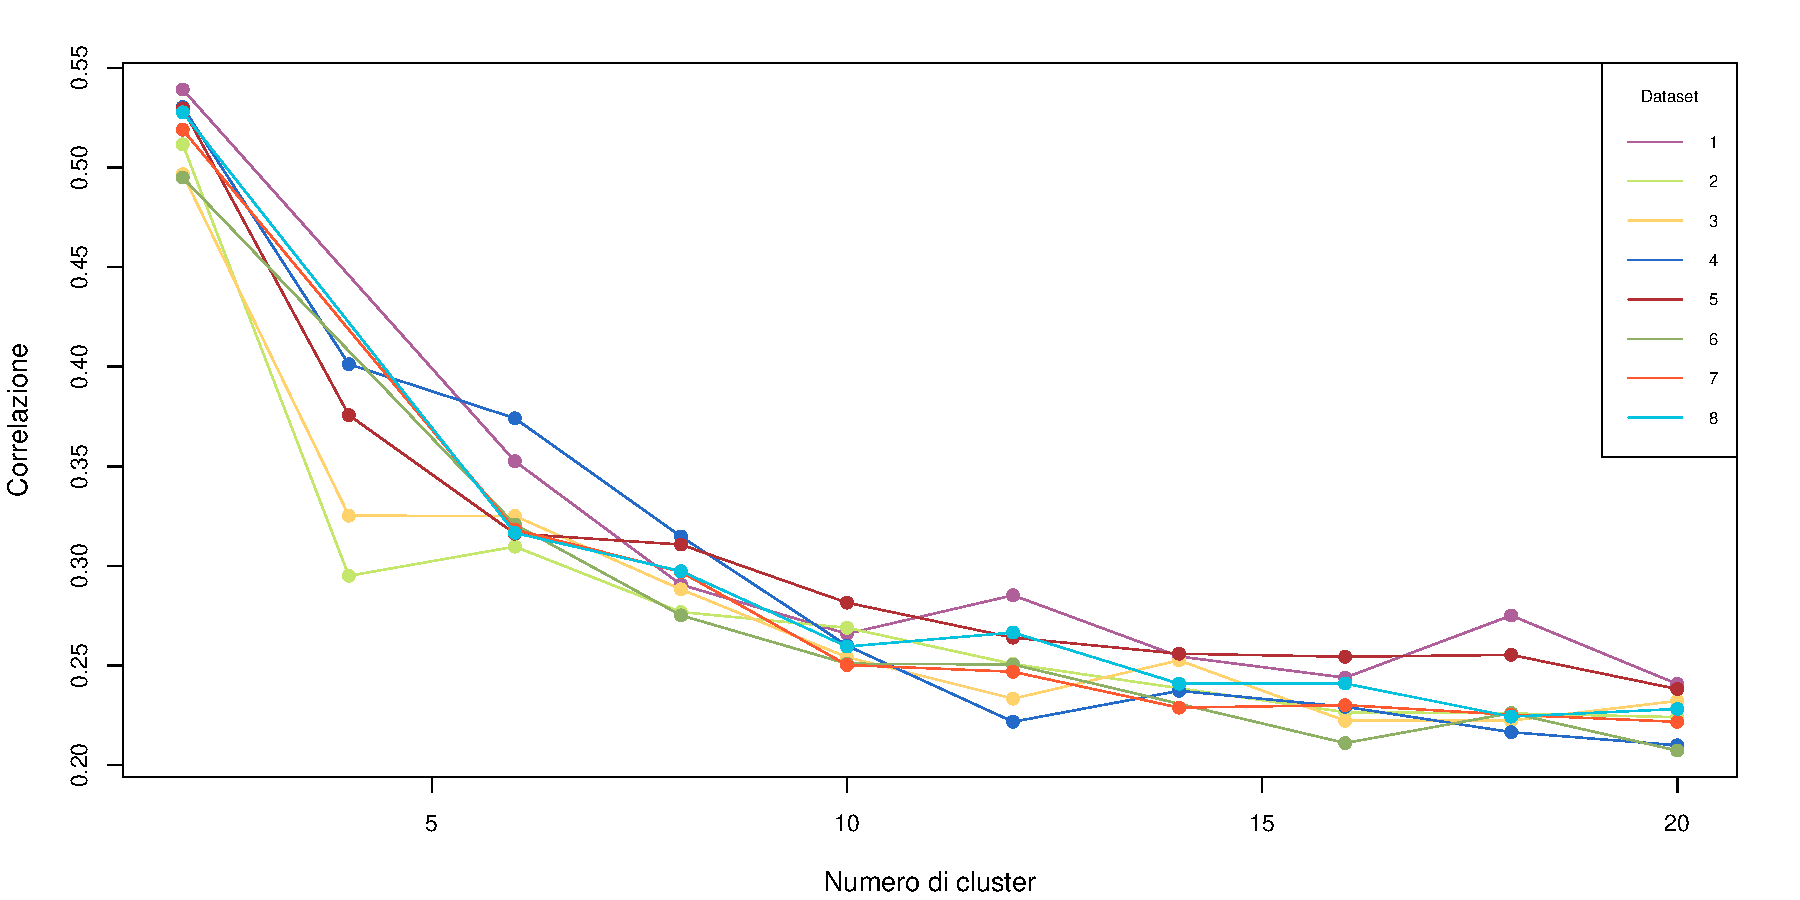
\includegraphics[width=\textwidth]{pictures/LAC/H1_1500.pdf}
                %\caption{h = 1}
                %\label{fig:h1_lac_correlation_1500}
        \end{subfigure}
        
        \begin{subfigure}[b]{0.85\textwidth}
                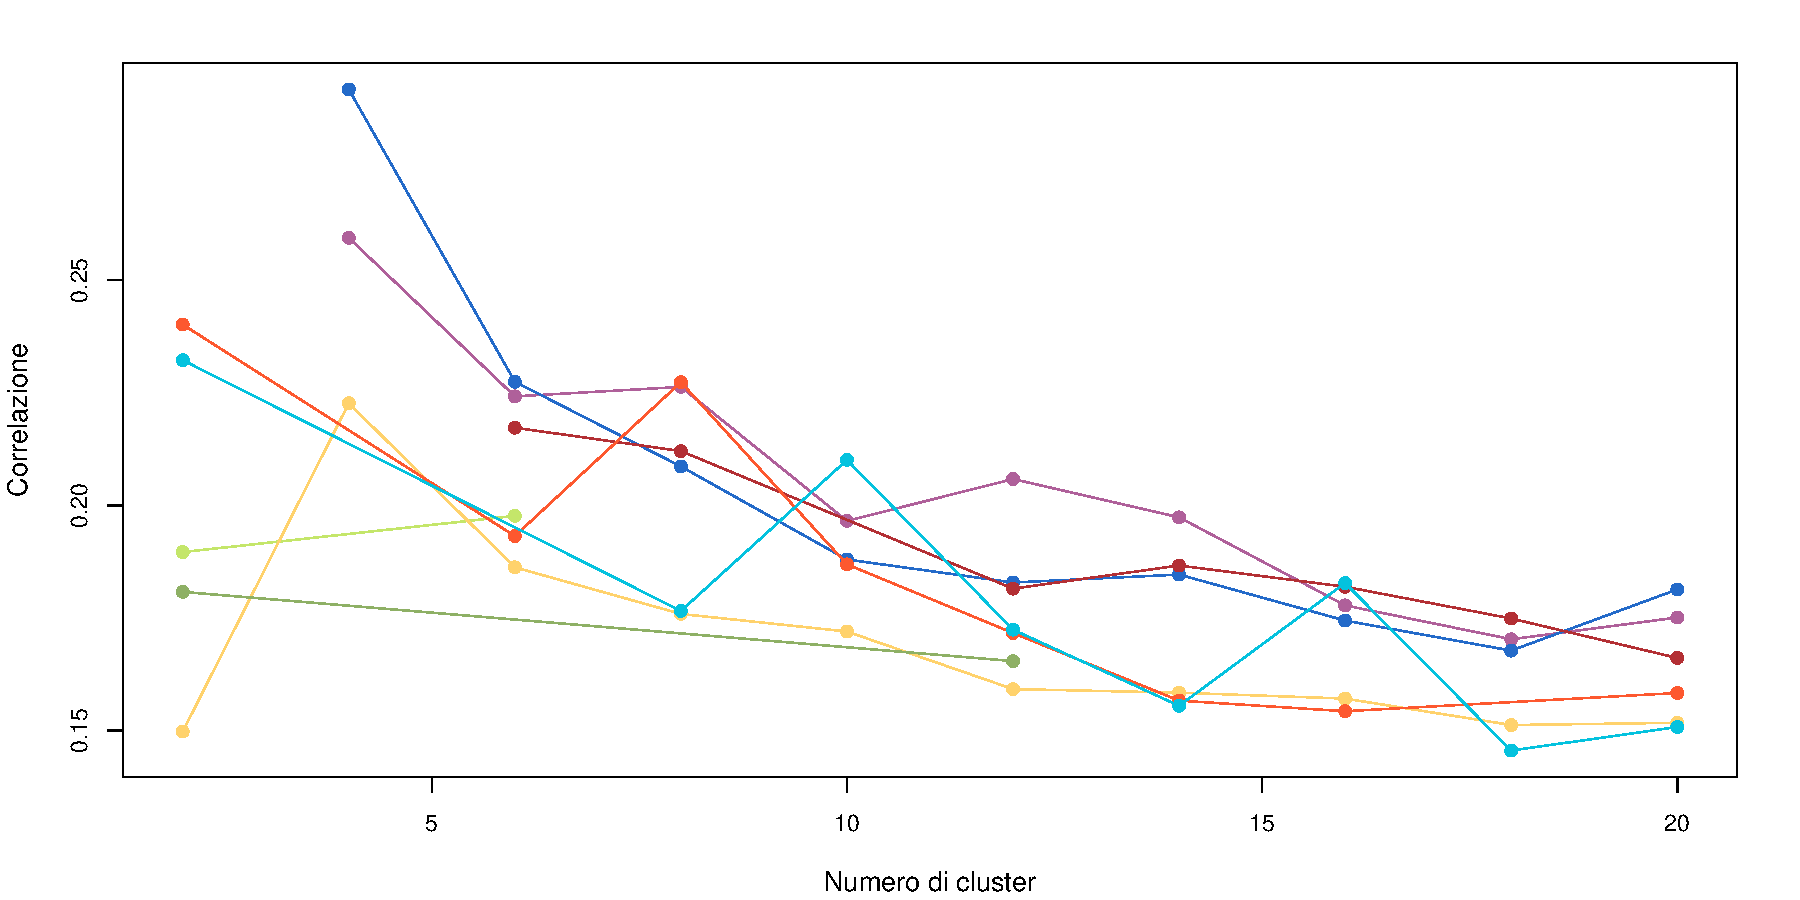
\includegraphics[width=\textwidth]{pictures/LAC/H2_1500.pdf}
                %\caption{h = 2}
                %\label{fig:h2_lac_correlation_1500}
        \end{subfigure}
        
        \begin{subfigure}[b]{0.85\textwidth}
                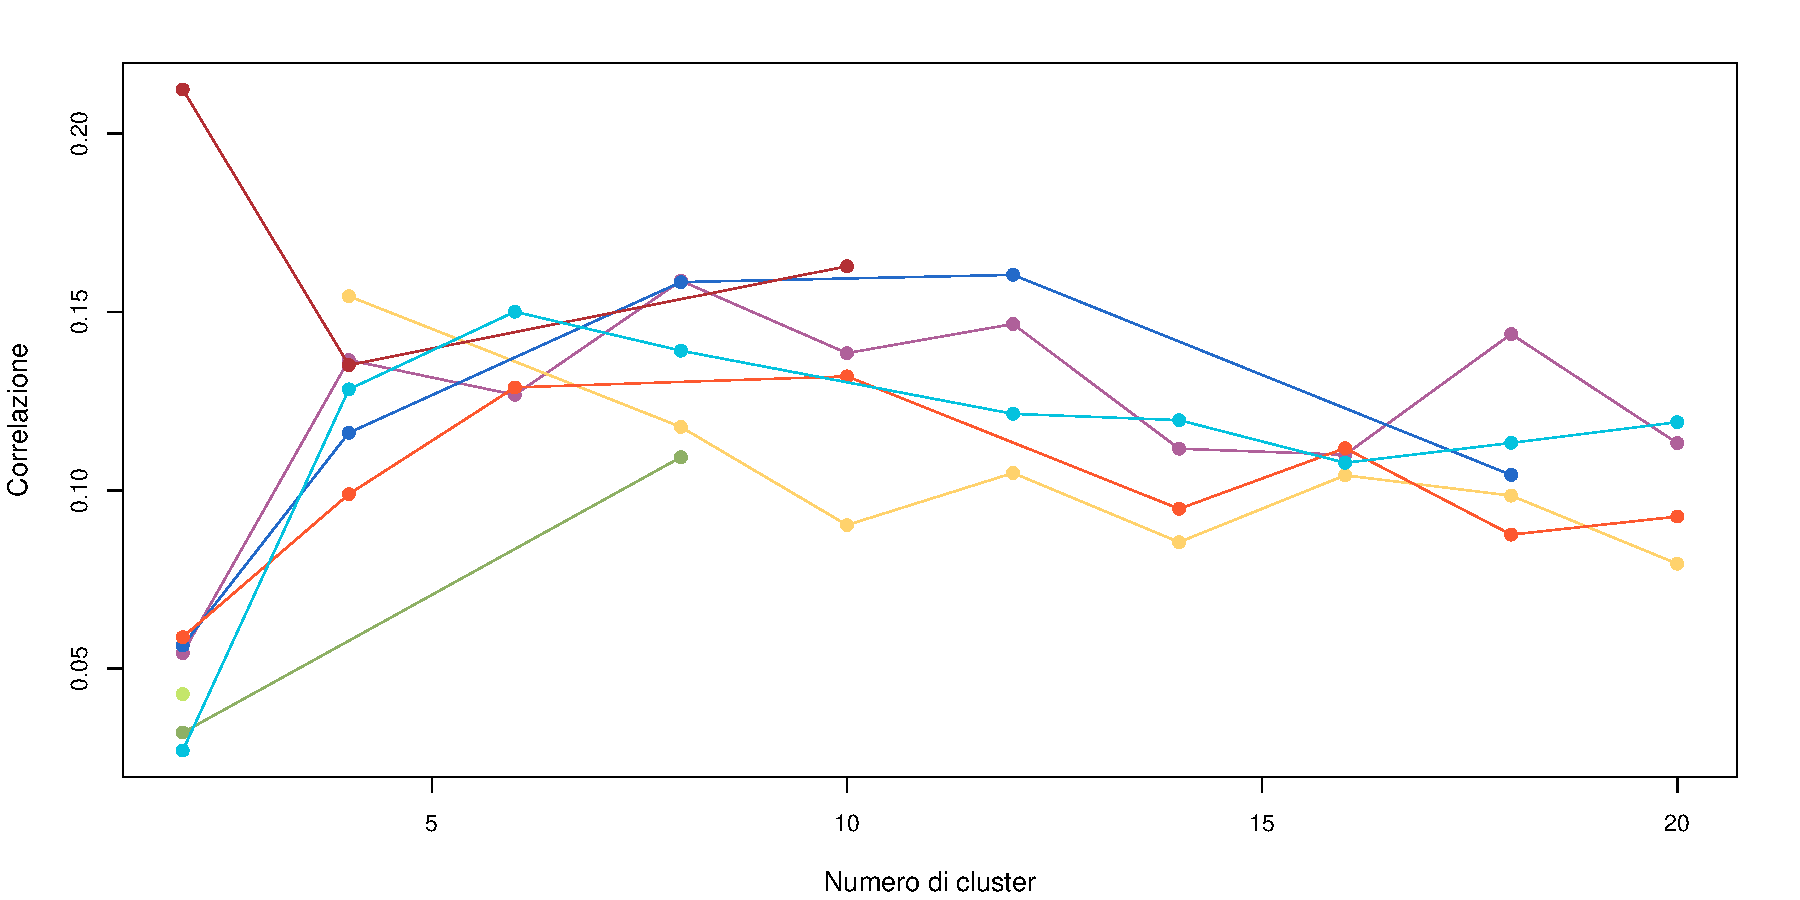
\includegraphics[width=\textwidth]{pictures/LAC/H3_1500.pdf}
                %\caption{h = 3}
                %\label{fig:h3_lac_correlation_1500}
        \end{subfigure}
        \caption{Prestazioni di LAC su campioni di 1500 nodi, rispettivamente per h=1, h=2 e h=3}\label{fig:lac_correlation_1500}
\end{figure}\\
\`E interessante osservare che, avendo fissato \textit{h}, campioni significativamente diversi del grafo completo mostrano l'evoluzione della prestazione al variare di \textit{k} � regolare, pur avendo considerato per questa analisi dei   (\autoref{table:omogeneita_1500}). Osservando \autoref{fig:lac_correlation_1500} (a), il digradare della correlazione al crescere di \textit{k} non � motivato da una penalizzazione delle soluzioni inutilmente complesse, poich� la correlazione misura unicamente la purezza e non la sintesi del clustering. Pertanto sembra essere una \\
Ricordiamo che nel calcolo della correlazione, la similarit� � calcolata nello spazio completo degli attributi: pertanto appare in qualche modo paradossale che richiedere una soluzione con sottospazi di dimensione crescente, che quindi si avvicinano di pi� alla percezione delle distanze considerata per la correlazione, produca soluzioni di qualit� via via peggiore. Questa tendenza pu� essere chiaramente esaminata in \autoref{fig:h_by_dataset}.
\begin{figure}[h]
    \centering
    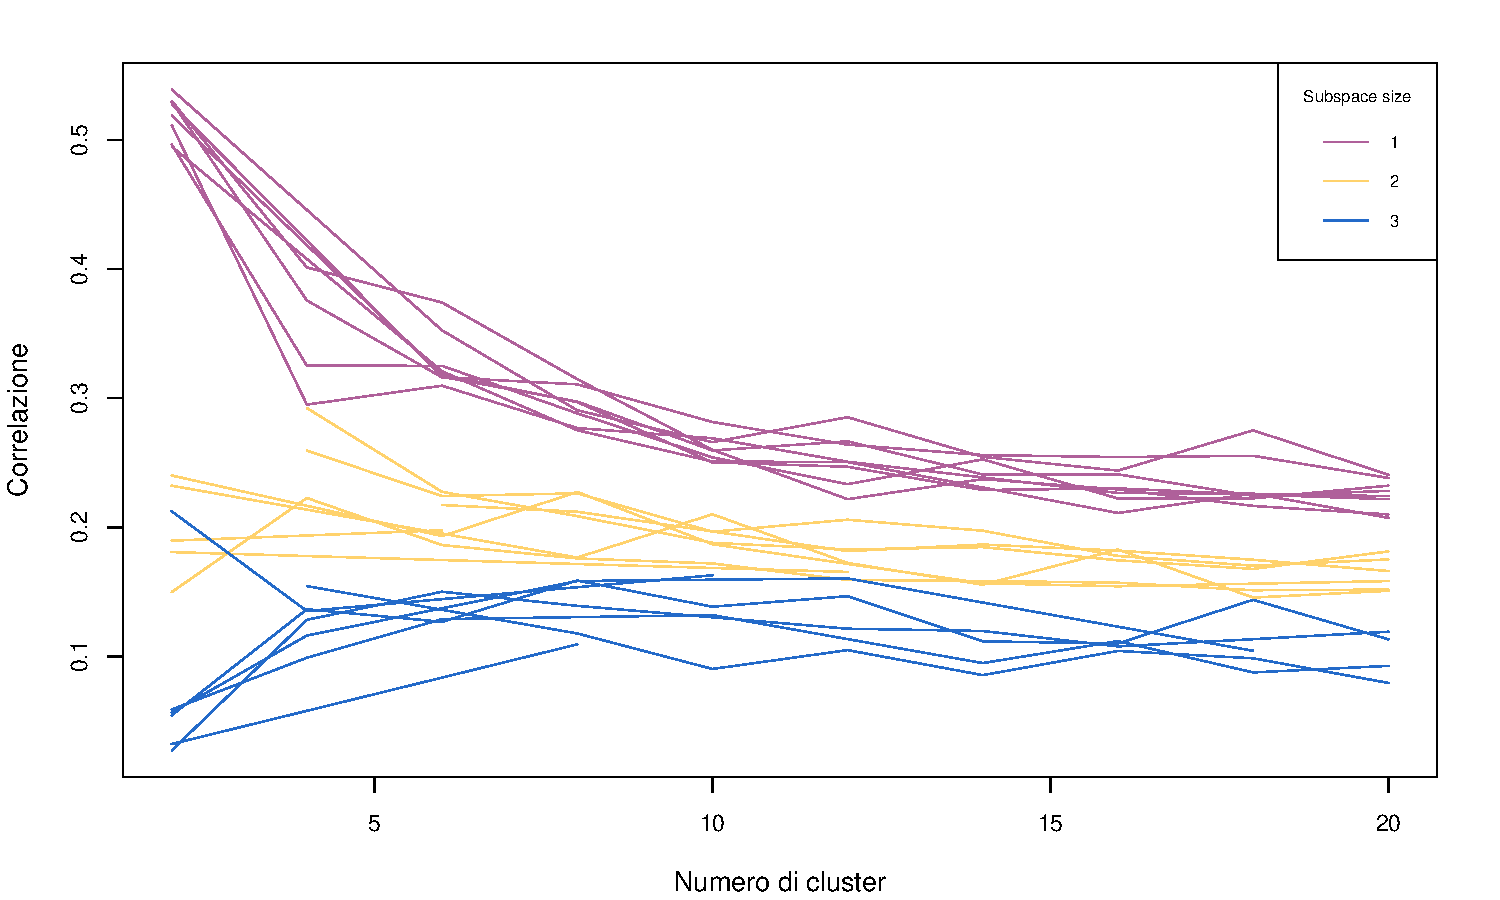
\includegraphics[width=0.95\textwidth]{pictures/LAC/H_by_Dataset.pdf}
    \caption{Correlazione al variare del parametro h}
	\label{fig:h_by_dataset}
\end{figure}\\
LAC mostra dei tempi di computazione estremamente dipendenti dalla dimensione del dataset. Questa dipendenza non altera significativamente il tempo di esecuzione di una singola iterazione dell'algoritmo--- che ricordiamo essere $O(kDN)$---ma incide sul numero di iterazioni prima della convergenza.\\
Le condizioni iniziali dell'algoritmo, come ad esempio la scelta dei centroidi, non sembrano avere rilievo nei tempi di convergenza, come si nota in \autoref{fig:lac_boxplots}. Fissata la dimensione h dei sottospazi, ripetute esecuzioni dell'algoritmo per un dato k hanno prodotto tempi di esecuzione pressoch� stazionari, n� le oscillazioni sono dovute ad ad un diverso ritmo di convergenza, poich� il numero di iterazioni � risultato costante fra le diverse rilevazioni. Un altro dettaglio di interesse � che il la rapidit� di convergenza non sembra correlata alla dimensione \textit{k} del clustering.
\begin{figure}[h]
        \centering
        \begin{subfigure}[b]{0.3\textwidth}
                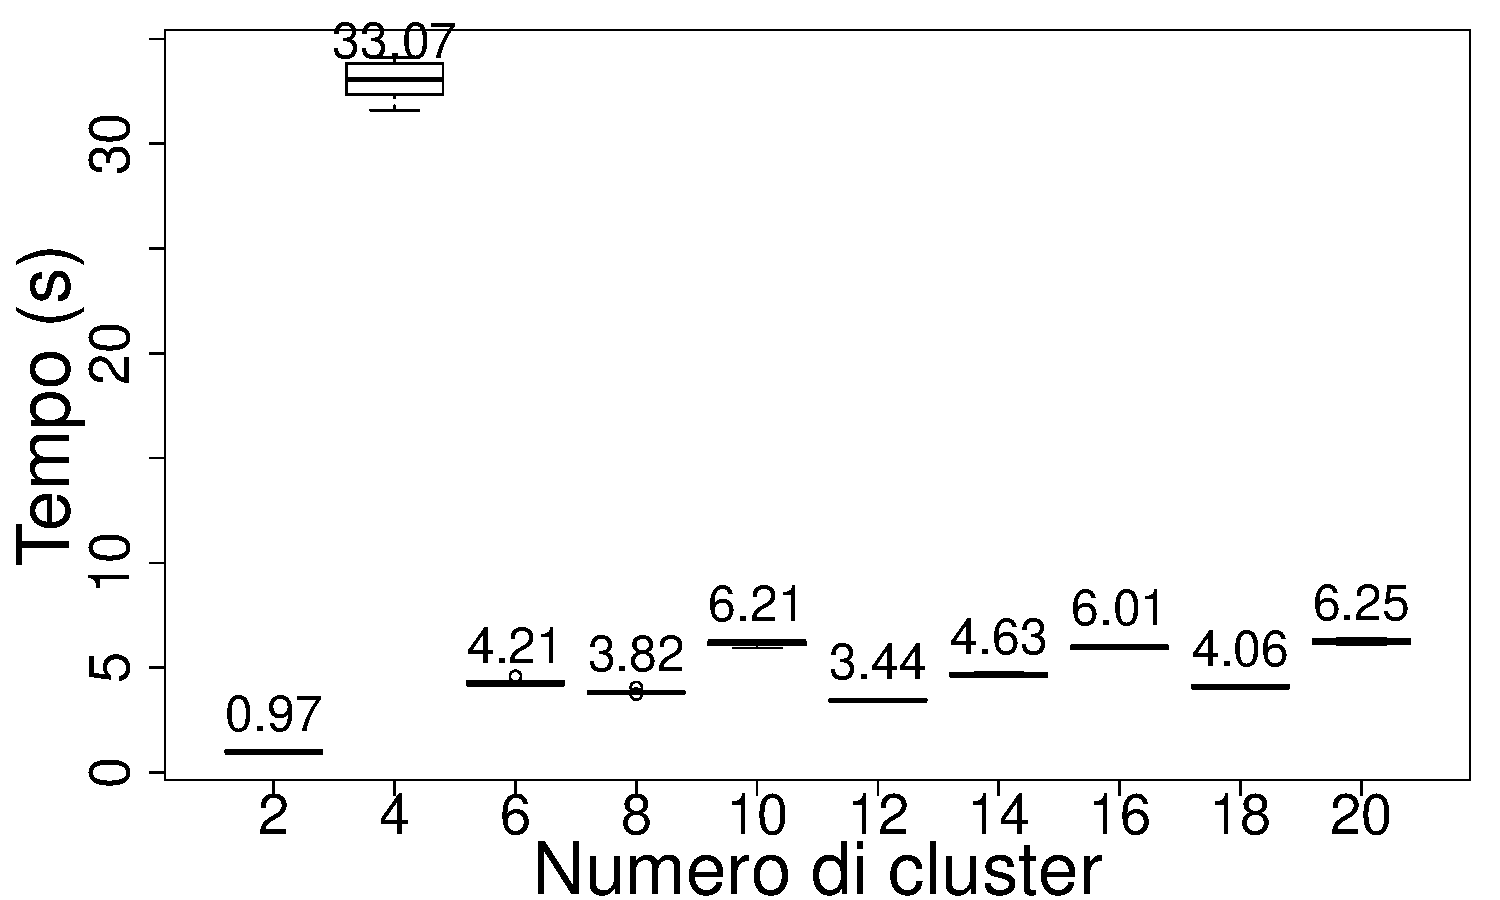
\includegraphics[width=\textwidth]{pictures/LAC/H1_Time_Boxplot_large.pdf}
                \caption{h = 1}
                \label{fig:h1_lac_boxplot}
        \end{subfigure}%
        ~
        \begin{subfigure}[b]{0.3\textwidth}
                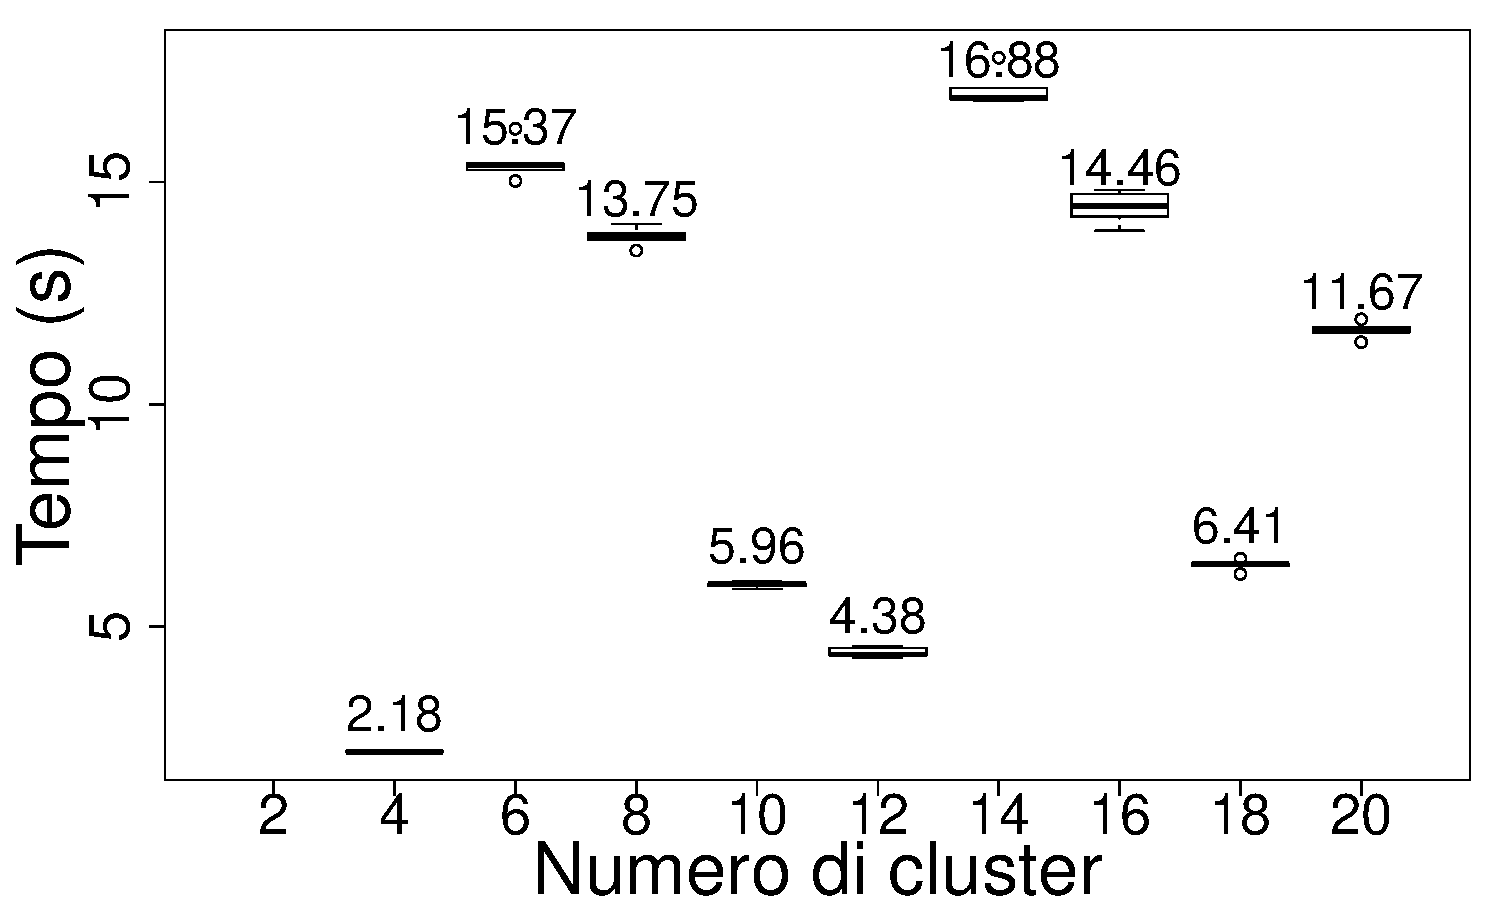
\includegraphics[width=\textwidth]{pictures/LAC/H2_Time_Boxplot_large.pdf}
                \caption{h = 2}
                \label{fig:h2_lac_boxplot}
        \end{subfigure}
        \begin{subfigure}[b]{0.3\textwidth}
                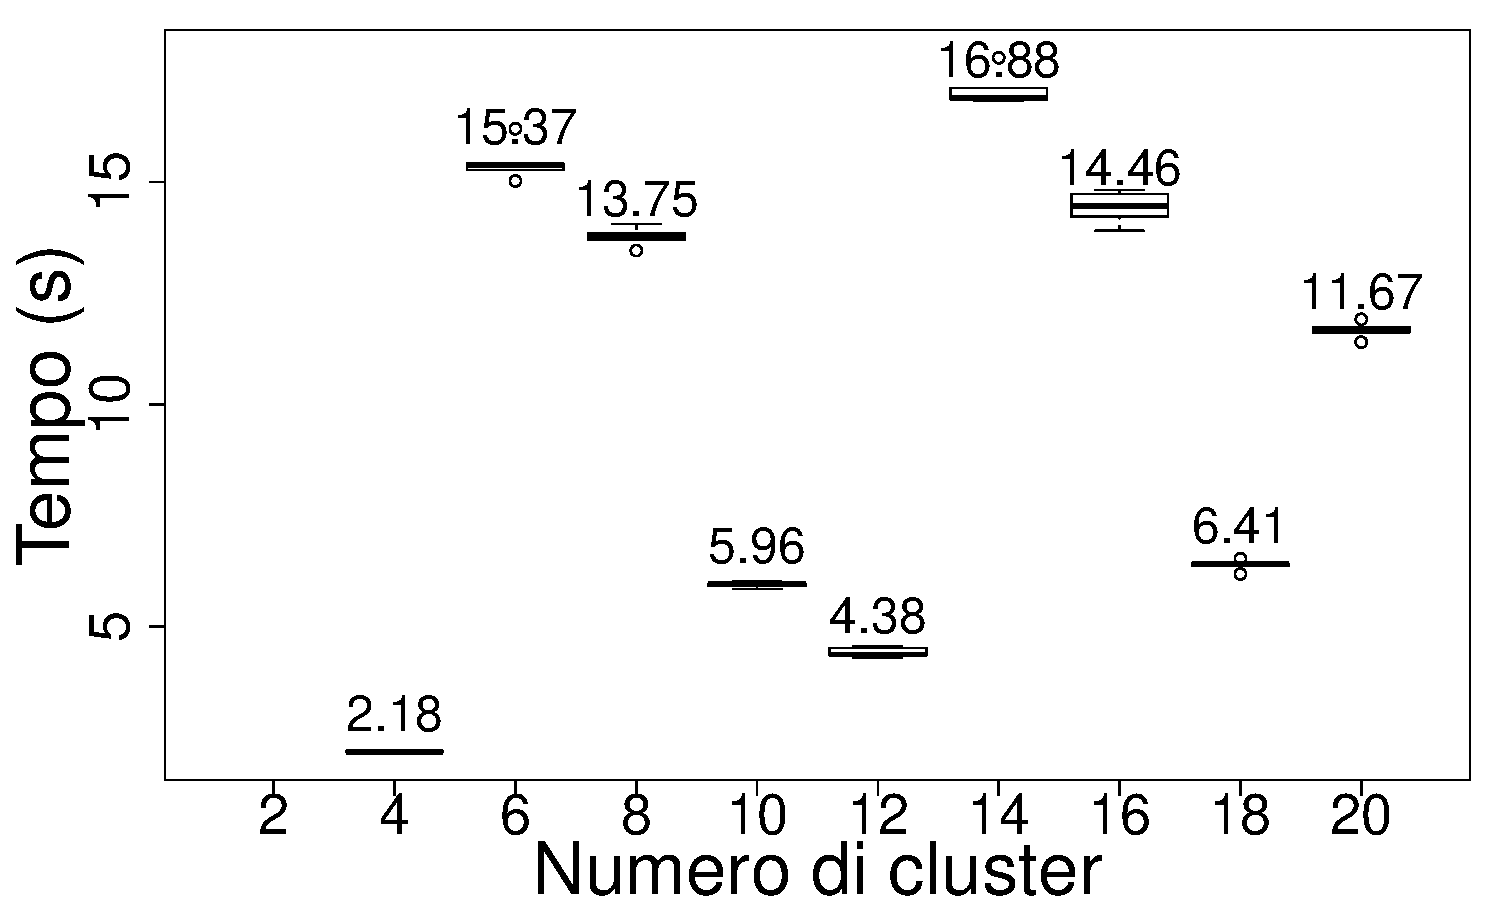
\includegraphics[width=\textwidth]{pictures/LAC/H2_Time_Boxplot_large.pdf}
                \caption{h = 3}
                \label{fig:h3_lac_boxplot}
        \end{subfigure}
        \caption{Variabilit� dei tempi di esecuzione di LAC sul dataset 1}\label{fig:lac_boxplots}
\end{figure}\\
Durante gli esperimenti abbiamo constatato che l'algoritmo richiede tempi esponenzialmente pi� lunghi di convergenza all'aumentare della dimensione del campione. Abbiamo riportato i tempi registrati su dataset di circa 1500 nodi in \autoref{fig:lac_time_1500}.
\begin{figure}[h]
        \centering
        \begin{subfigure}[b]{0.9\textwidth}
                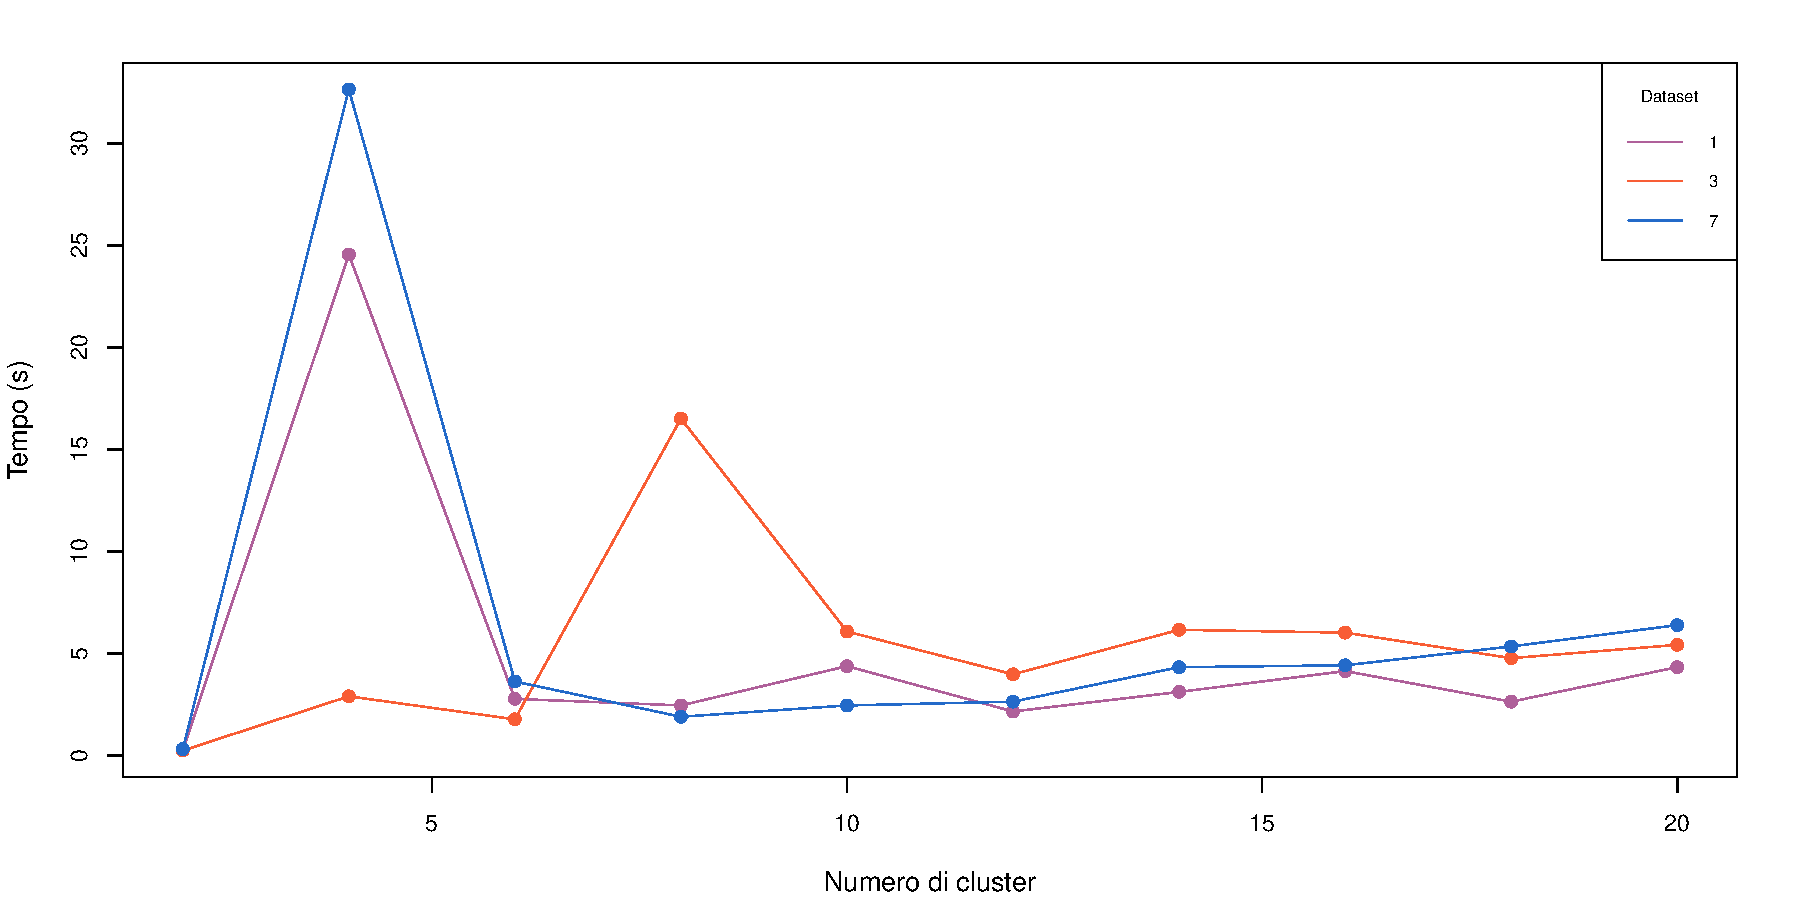
\includegraphics[width=\textwidth]{pictures/LAC/H1_1500_Time.pdf}
                %\caption{h = 1}
                %\label{fig:h1_lac_time_1500}
        \end{subfigure}
        
        \begin{subfigure}[b]{0.9\textwidth}
                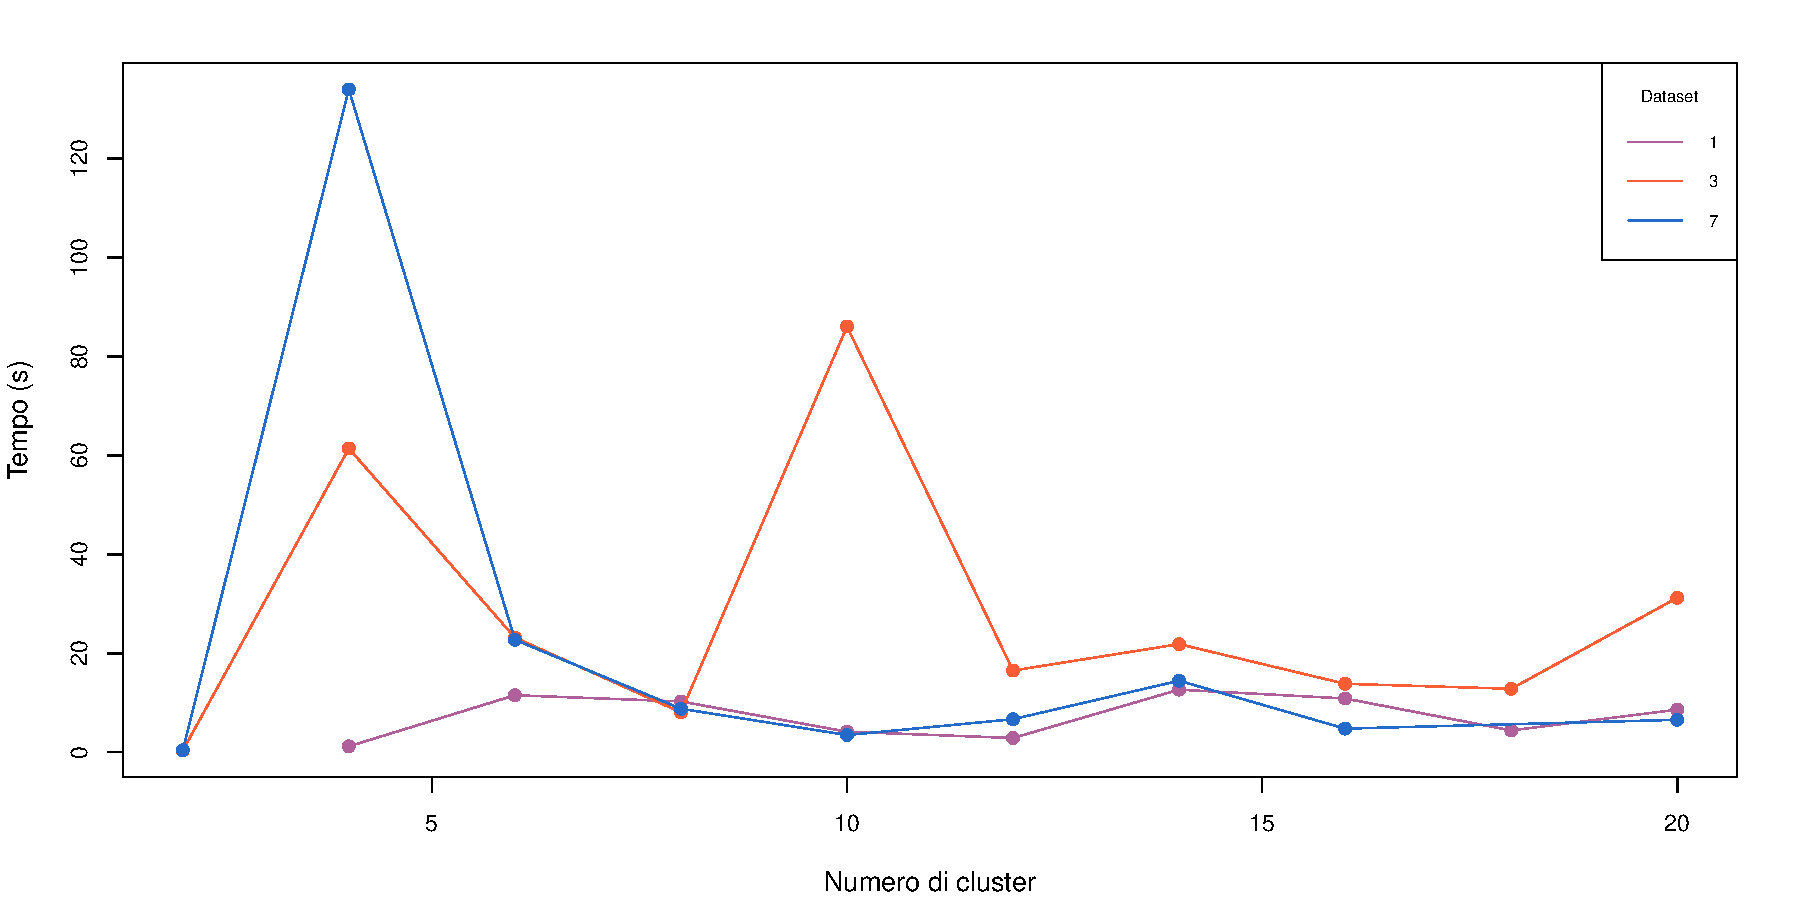
\includegraphics[width=\textwidth]{pictures/LAC/H2_1500_Time.pdf}
                %\caption{h = 2}
                %\label{fig:h2_lac_time_1500}
        \end{subfigure}
        
        \begin{subfigure}[b]{0.9\textwidth}
                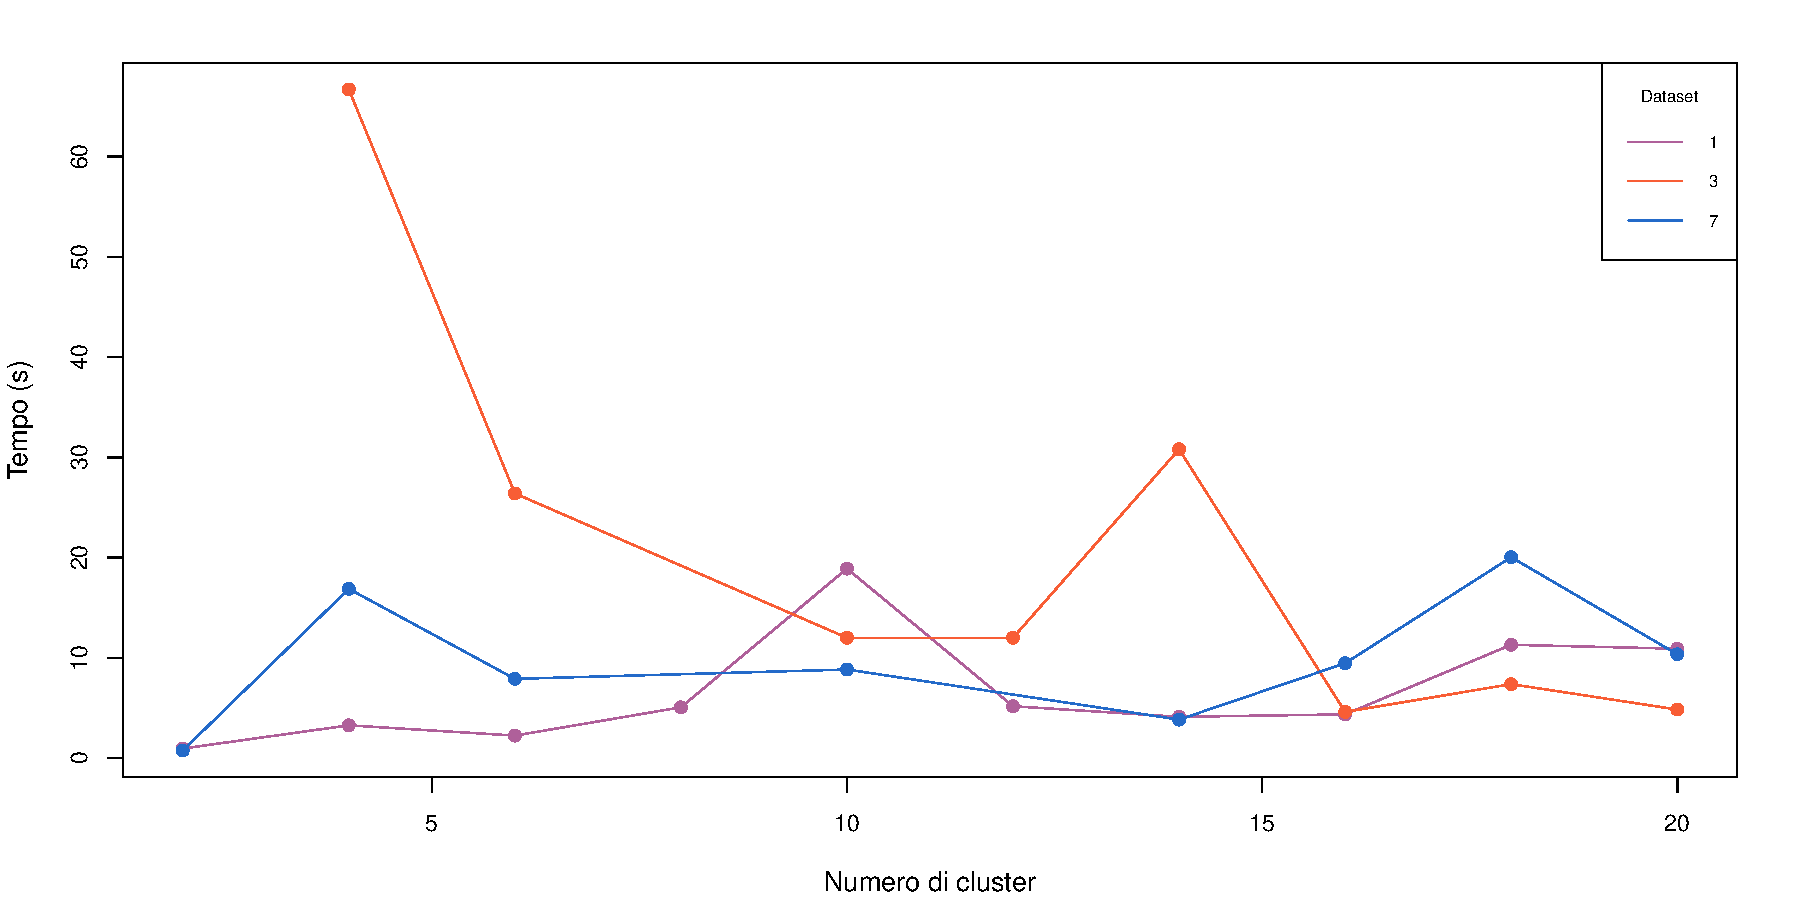
\includegraphics[width=\textwidth]{pictures/LAC/H3_1500_Time.pdf}
                %\caption{h = 3}
                %\label{fig:h3_lac_time_1500}
        \end{subfigure}
        \caption{Tempi di esecuzione di LAC su campioni del grafo di 1500 nodi, rispettivamente per h=1, h=2 e h=3}\label{fig:lac_time_1500}
\end{figure}\\
Nel passare a campioni di 3000 elementi, il tempo richiesto dall'algoritmo � peggiorato sensibilmente (\autoref{fig:lac_time_3000}), accentuandosi al crescere del parametro \textit{h}. Non � stato possibile procedere oltre questa dimensione poich�, in svariati tentativi su dataset di 6000 utenti, l'algoritmo non ha mai raggiunto la convergenza dopo numerose ore di elaborazione. Sebbene gli autori abbiano fornito la prova teorica della convergenza dell'algoritmo, nella pratica i tempi di esecuzione sono incompatibili con il nostro scenario.
\begin{figure}[h]
    \centering
    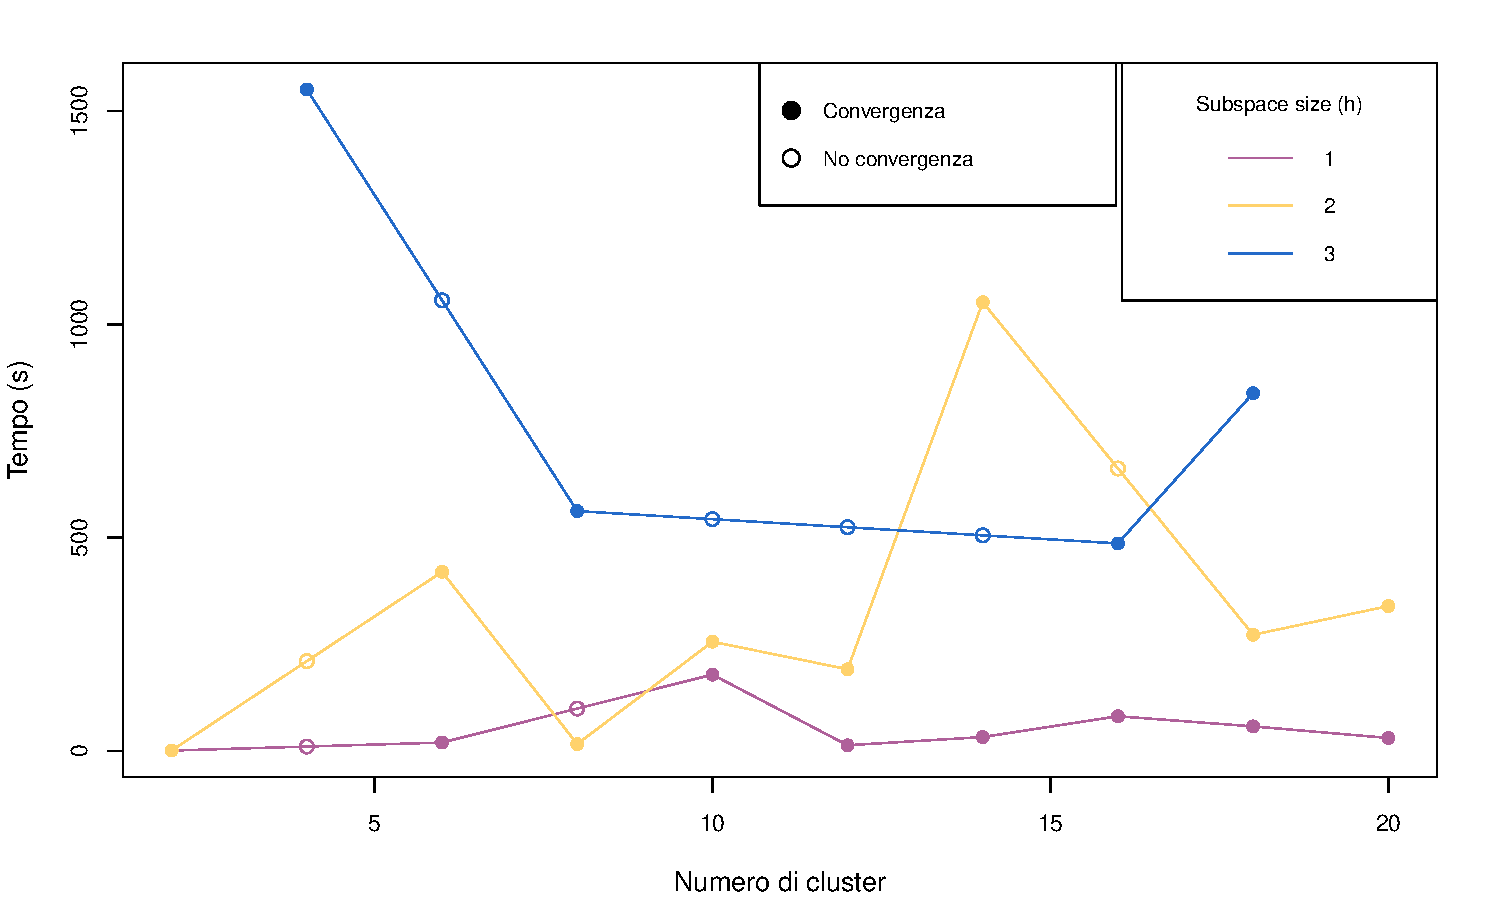
\includegraphics[width=0.95\textwidth]{pictures/LAC/H_by_Dataset_Time_3000.pdf}
    \caption{Tempi di esecuzione di LAC (3000 nodi)}
	\label{fig:lac_time_3000}
\end{figure}\\

%\begin{figure}[h]
%    \centering
%    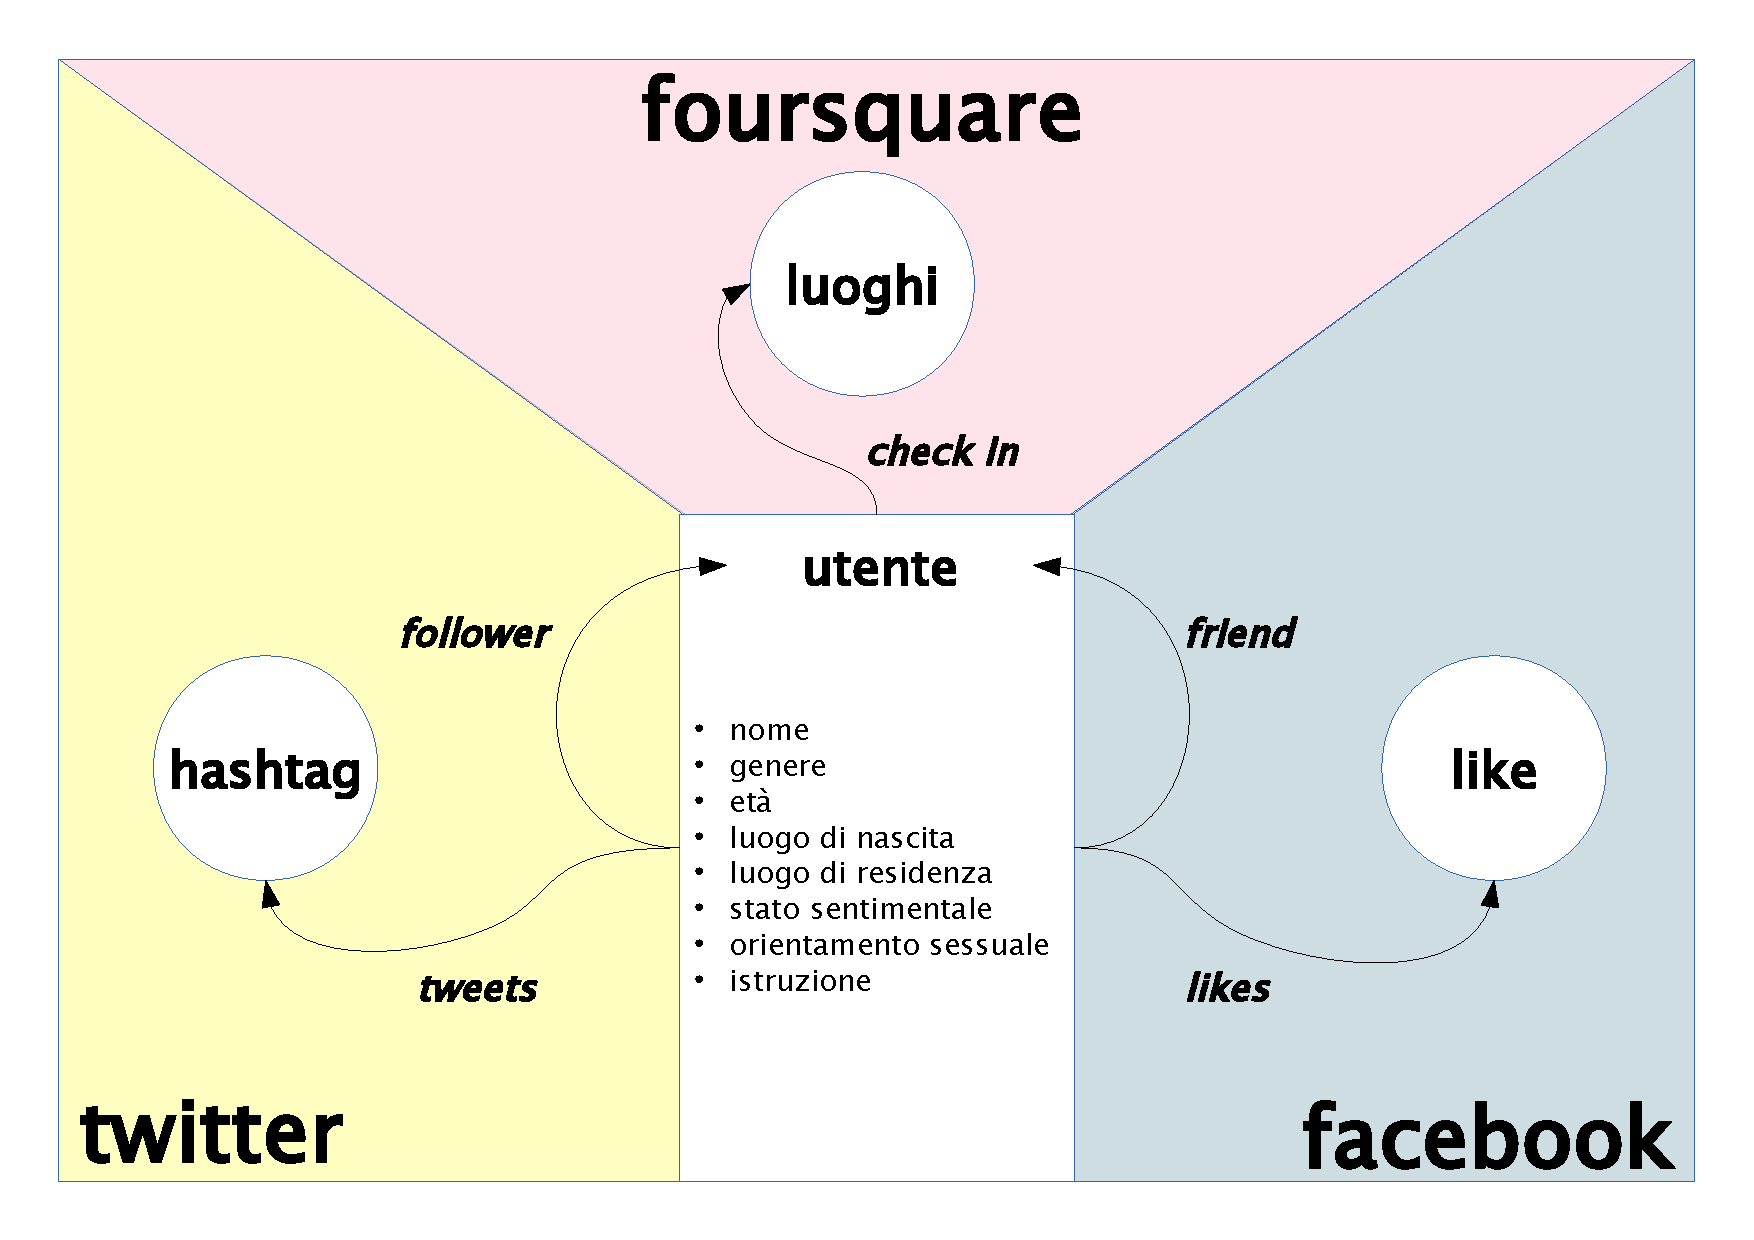
\includegraphics[width=0.95\textwidth]{pictures/modello_dati.pdf}
%    \caption{Modello dei dati}
%    \label{fig:modello_dati}
%\end{figure}

\section{ORCLUS}

\section{MOC}

\section{CESNA}

\section{BAGC}

